\documentclass[11pt, oneside]{article} 
\usepackage{geometry}
\geometry{letterpaper} 
\usepackage{graphicx}
	
\usepackage{amssymb}
\usepackage{amsmath}
\usepackage{parskip}
\usepackage{color}
\usepackage{hyperref}

\graphicspath{{/Users/telliott_admin/Dropbox/Tex/png/}}
% \begin{center} 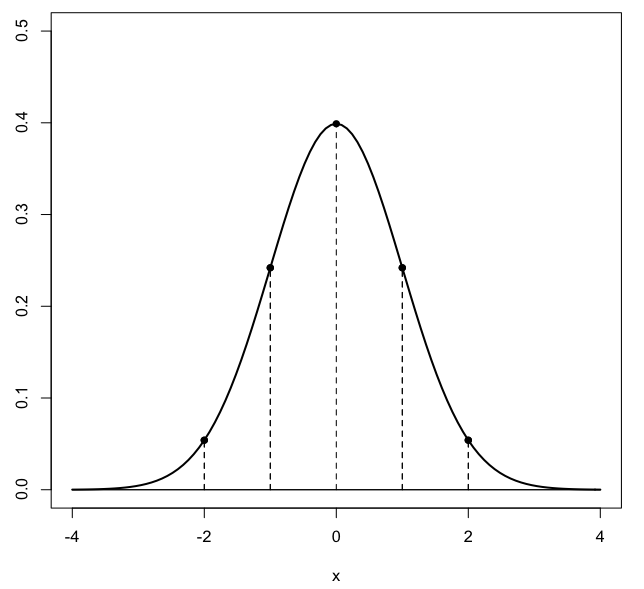
\includegraphics [scale=0.4] {gauss3.png} \end{center}

\title{The triangle inequality}
\date{}

\begin{document}
\maketitle
\Large
\subsection*{absolute value:  definition}
\[ |x| = x, \ \ \ \ x \ge 0 \]
\[ |x| = -x, \ \ x < 0 \]

\subsection*{triangle inequality theorem}
We will prove that 
\[ |x + y| \le |x| + |y| \] 
as well as some corollaries and a related theorem:
\[ |x - y| = |y - x| \]
\[ |x - y| \le |x - z| + |z - y| \]
\[ |xy| = |x| \ |y| \]

\subsection*{theorem}
\[ |x + y| \le |x| + |y| \]

Just to be clear, this holds regardless of the sign of $x$ and $y$.

\subsection*{proof}
Let $m > n > 0$.  If $n > m$, just switch $x$ and $y$.  We deal with the case $m=n$ and $x,y$ of different signs in the last part.

$\bullet$  $x$ and $y$ with the same sign

$\circ$  $x = m, y = n$
\[ |x + y| = |m + n| = m + n \]
\[ m + n = |m| + |n| = |x| + |y| \]
$\circ$  $x = -m, y = -n$
\[ |x + y| = |-m - n| = |-(m + n)| = m + n \]
\[ m + n = |-m| + |-n| = |x| + |y| \]

$\bullet$  one of $x,y$ is equal to zero

$\circ$  $x = m, y = 0$
\[ |x + y| = |m + 0| = |m| = m \]
\[ m = m + 0 = |m| + |0| = |x| + |y| \]
$\circ$  $x = -m, y = 0$
\[ |x + y| = |-m + 0| = |-m| = m \]
\[ m = m + 0 = |-m| + |0| = |x| + |y| \]

$\bullet$  one of $x,y$ is less than zero

Here we see the inequality.  Let $p = m - n$ (we assume $m > n$ so $p > 0$).
\[ p = m - n \]
\[ p < p + 2n \]
\[ p < m + n \]

$\circ$  $x = -m, y = n$
\[ |x + y| = |-m + n| = |-p| = p < m + n \]
\[ m + n = |-m| + |n| = |x| + |y| \]
so
\[ |x + y| < |x| + |y| \]

$\circ$  $x = m, y = -n$
\[ |x + y| = |m - n| = |p| = p < m + n \]
\[ m + n = |m| + |-n| = |x| + |y| \]
so
\[ |x + y| < |x| + |y| \]

$\circ$  For unequal signs, suppose that $m=n$.  Then $x = m, y = -m$.
\[ |x + y| = |m + -m| = 0 < |m| + |-m| = |x| + |y| \]

$\square$

\subsection*{accessory theorem:  multiplication}
\[ |xy| = |x| \ |y| \]

Obviously true for equal signs or one of $x,y$ equal to zero.  For different signs
\[ |xy| = |(-m)n| = |-mn| = mn = |-m| \ |n| = |x| \ |y| \]
$\square$

\subsection*{accessory theorem:  change of sign}
\[ |x - y| = |y - x| \]

\subsection*{corollaries of the triangle theorem}
\[ |x - y| \le |x - z| + |z - y| \]
\[ |x - y| \ge |x| - |y| \]

\subsection*{theorem}
\[ |x - y| = |y - x| \]
\subsection*{proof}
Suppose that what is meant is $m,n > 0$ and $x = m, y =-n$.

$\circ$  $m > n$ so $m - n = p > 0$
\[ |x - y| = |m - n| = |p| = p \]
\[ |y - x| = |n - m| = |-p| = p \]
so
\[ |x - y| = |y - x| \]
Having $n > m$ does not change the argument

$\circ$  $n > m$ so $m - n = -p < 0$
\[ |x - y| = |m - n| = |-p| = p \]
\[ |y - x| = |n - m| = |p| = p \]

\subsection*{theorem}
\[ |x - z|  \le |x - y| + |z - y| \]

Suppose that what is meant is $x,y > 0$.  It doesn't matter since the triangle theorem holds regardless of the signs of the two terms.

\subsection*{proof}
Start with the triangle inequality
\[ |x + y| \le |x| + |y| \]

Replace $x$ by $x-y$ and $y$ by $y-z$ 
\[ |x-y + y-z| \le |x-y| + |y-z| \]
\[ |x - z|  \le |x - y| + |z - y| \]

We can substitute letters if you prefer something different
\[ |x - y|  \le |x - z| + |y - z| \]

Geometrically, the largest distance is equal to the other two together.  Any other single distance is less than the sum of the remaining two.

\begin{center} 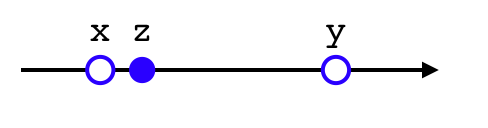
\includegraphics [scale=0.4] {3points.png} \end{center}
\[ |x - y| \le |x - z| + |z - y| \]

We can switch the order for any term by the first corollary above
\[ |x - y|  \le |x - z| + |y - z| \]
goes to
\[ |x - y|  \le |x - z| + |z - y| \]

\subsection*{theorem}
\[  |x - y| \ge |x| - |y|  \]

\subsection*{proof}
\[ |x + y| \le |x| + |y| \]

Replace $x$ by $x - y$
\[ |x| \le |x - y| + |y| \]
\[ |x - y| \ge |x| - |y| \]

\end{document}